% 研究の背景、動機、目的を述べる。
% 論文全体の見通しを示す。何章で何を述べるかを明確にする。

% 研究の背景
% - 生体と温度の関係
% - TRPチャネル全体について
%   - TRPV1-6について
%   - TRPMについて
% - TRPV3について
%   - TRPV3の構造と機能
%
% 研究の目的
% - TRPV3を機能させるにいたるネットワークを明らかにする
% - TRPV3の構造と機能の関係を明らかにする
%
% 研究の方法と結果(簡単に)
%
% 研究の結論(簡単に)
%
% 論文の構成

\section{はじめに}

\section{TRPV3チャネル}
% まずTRPチャネルとTRPVチャネルについてそれぞれ1パラグラフ程度で説明した後、TRPV3チャネルについて説明する。
% TRPチャネル
TRPV3チャネルはTRP(Transient Receptor Potential)チャネル、その中でもTRPVチャネルの一種である。
TRPチャネルはカチオンチャネルのスーパーファミリーで、配列相同性はまちまちながらも似通った構造を持っており、
そのどれもが外界からの刺激を受けて応答するのに関与している。\autocite{venkatachalam_trp_2007}

% FIXME: TRPVの歴史について記述
% FIXME: TRPV5,6についても書く
TRPVチャネルファミリーはTRPV1,2,3,4,5,6に分類されており、
そのうち1-4は感知する温度や温度に対する応答が異なるものの、温度感知性を持つ。\autocite{baylie_trpv_2011}

% TRPV3チャネル概要
その中でもTRPV3チャネルは、温度T = 36-39℃で活性化する温度感知性を持つ。\autocite{baylie_trpv_2011,xuTRPV3CalciumpermeableTemperaturesensitive2002}
ヒトのゲノムデータベースを探索することで、多くのTRPV3チャネルが報告されてきた。\autocite{smithTRPV3TemperaturesensitiveVanilloid2002, xuTRPV3CalciumpermeableTemperaturesensitive2002, peier_heat-sensitive_2002}
TRPV3は人やマウスの神経細胞や肌に存在することが知られており、肌に対する外部からの物質や内部からの物資、熱によって活性化される。% TODO: 出展
% 閲覧注意: citeした3報。
% Recurrent... -> Gly573Ser
% exome... -> 3例で Gly573Ser, 1例ずつGly573Cys, Trp692Gly
また、TRPV3が肌でこれらの刺激を感受するため、肌の痛みや「かゆみ」などの感覚を与えるほか、
TRPV3遺伝子の変異はOlmsted syndromeという遺伝性皮膚疾患を引き起こす。\autocite{lin_exome_2012,lai-cheong_recurrent_2012,nilius_trpv_2013}
TRPV3は構造が明らかになる前から、活性・非活性を膜間を流れる電流によって検出することで、活性化条件を特定する研究が行われてきた。
\autocite{smithTRPV3TemperaturesensitiveVanilloid2002,xuTRPV3CalciumpermeableTemperaturesensitive2002,nadezhdinStructuralMechanismHeatinduced2021,chung_2-aminoethoxydiphenyl_2004}
% FIXME: 本当はTRPV3の性質についてもう少し詳しく書きたい。
% FIXME: 時間があればパラグラフを分けてもいい。
TRPV3は他のTRPチャネルに対して特異的な点として、温度刺激を繰り返し与えることによりイオンチャネルとしての活性が高まる。
\autocite{peier_heat-sensitive_2002,chung_2-aminoethoxydiphenyl_2004,liu_hysteresis_2011}

% 機能と構造について説明
TRPV3は単量体は790個程度のアミノ酸残基で構成された膜タンパク質であり、ホモ4量体を形成する。(図\ref{fig:trpv3})

\begin{figure}
  \centering
  \begin{subfigure}{0.4\textwidth}
    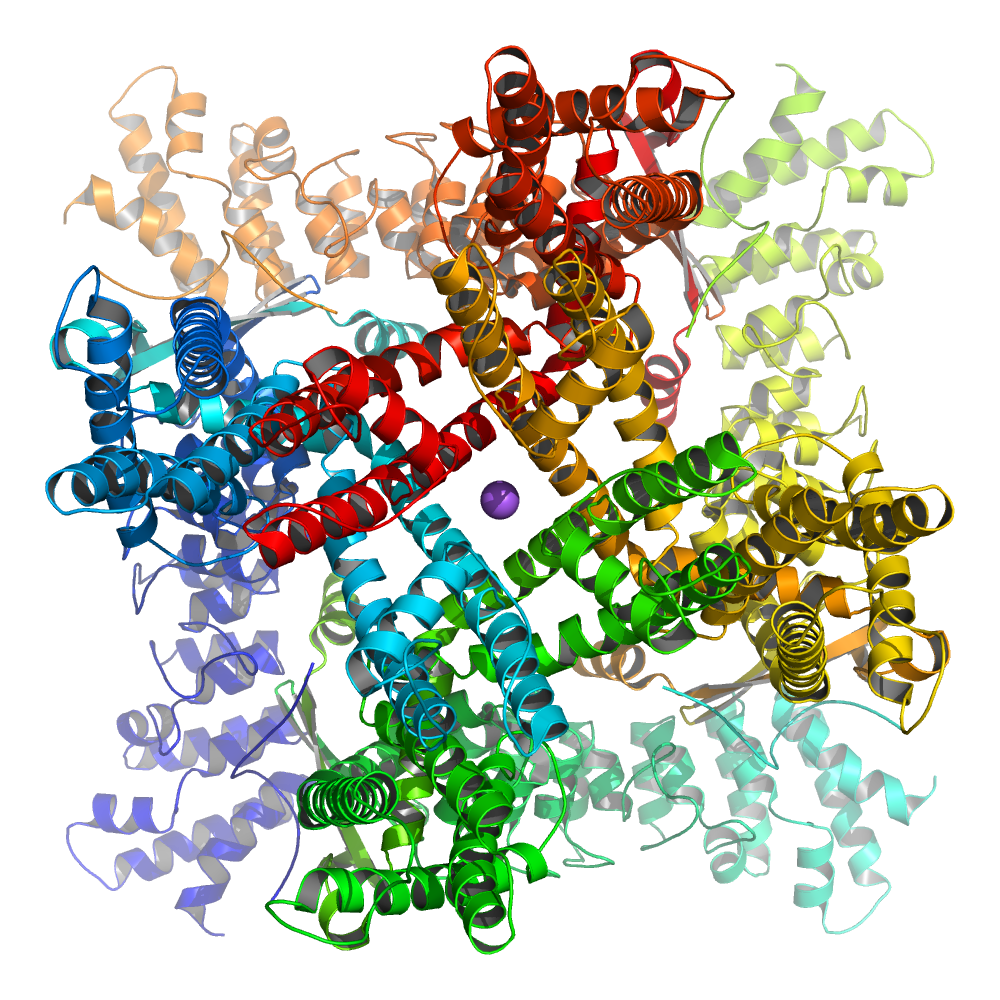
\includegraphics[width=\textwidth]{trpv3}
    \caption{膜の外側から見た様子}
    \label{fig:trpv3}
  \end{subfigure}
  \begin{subfigure}{0.4\textwidth}
    % FIXME: もっといいアングルや脂質を含めた様子がほしい。
    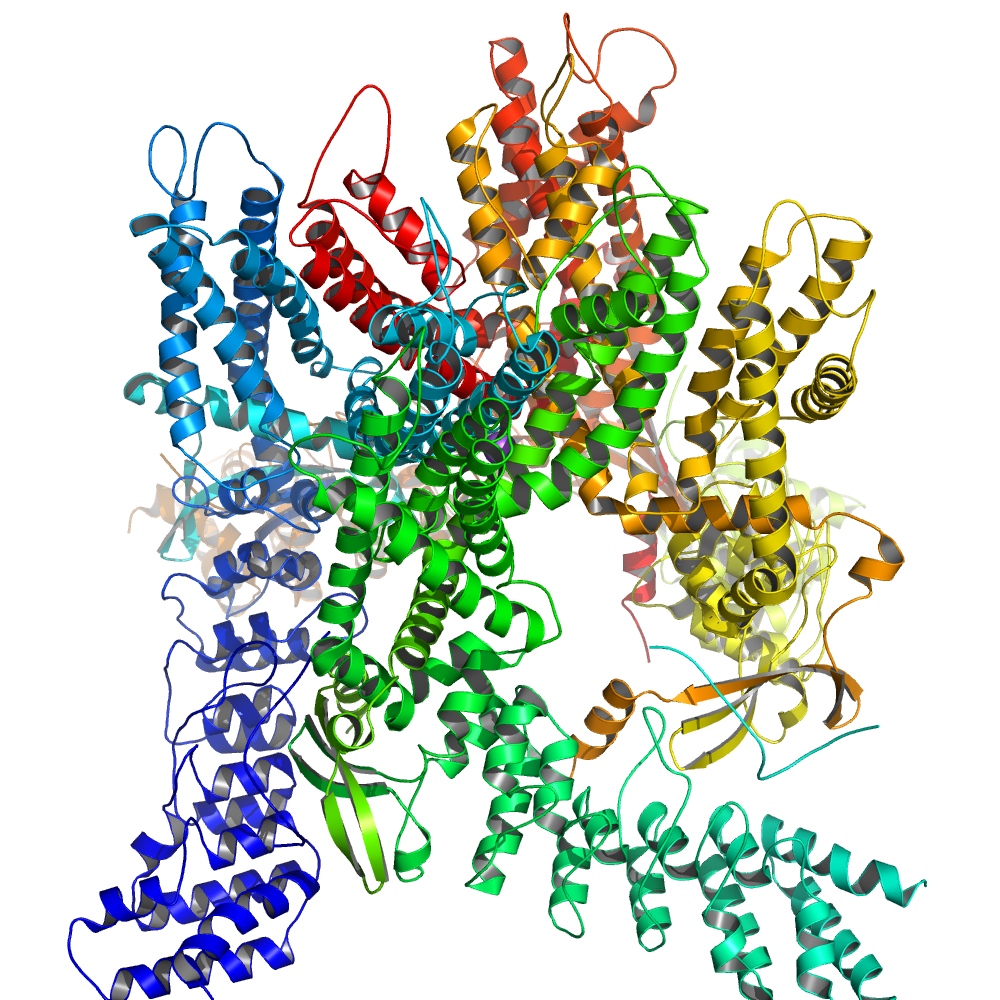
\includegraphics[width=\textwidth]{trpv3_angle}
    \label{fig:trpv3_angle}
  \end{subfigure}
  \caption{TRPV3の一つである7MIOの構造}
  \label{fig:trpv3_structures}
\end{figure}

残基数が多く構造が大きいためクライオ電子顕微鏡が登場するまでは一部のドメインのみの構造解析にとどまっていたが、
% https://www.rcsb.org/search?request=%7B%22query%22%3A%7B%22type%22%3A%22group%22%2C%22nodes%22%3A%5B%7B%22type%22%3A%22group%22%2C%22nodes%22%3A%5B%7B%22type%22%3A%22group%22%2C%22nodes%22%3A%5B%7B%22type%22%3A%22terminal%22%2C%22service%22%3A%22full_text%22%2C%22parameters%22%3A%7B%22value%22%3A%22TRPV3%22%7D%7D%2C%7B%22type%22%3A%22terminal%22%2C%22service%22%3A%22full_text%22%2C%22parameters%22%3A%7B%22value%22%3A%22TRPV%203%22%7D%7D%5D%2C%22logical_operator%22%3A%22and%22%7D%5D%2C%22logical_operator%22%3A%22and%22%2C%22label%22%3A%22full_text%22%7D%2C%7B%22type%22%3A%22group%22%2C%22nodes%22%3A%5B%7B%22type%22%3A%22group%22%2C%22nodes%22%3A%5B%7B%22type%22%3A%22group%22%2C%22nodes%22%3A%5B%7B%22type%22%3A%22terminal%22%2C%22service%22%3A%22text%22%2C%22parameters%22%3A%7B%22attribute%22%3A%22exptl.method%22%2C%22value%22%3A%22ELECTRON%20MICROSCOPY%22%2C%22operator%22%3A%22exact_match%22%7D%7D%5D%2C%22logical_operator%22%3A%22or%22%2C%22label%22%3A%22exptl.method%22%7D%5D%2C%22logical_operator%22%3A%22and%22%7D%5D%2C%22logical_operator%22%3A%22and%22%2C%22label%22%3A%22text%22%7D%5D%2C%22logical_operator%22%3A%22and%22%7D%2C%22return_type%22%3A%22entry%22%2C%22request_options%22%3A%7B%22paginate%22%3A%7B%22start%22%3A0%2C%22rows%22%3A25%7D%2C%22results_content_type%22%3A%5B%22experimental%22%5D%2C%22sort%22%3A%5B%7B%22sort_by%22%3A%22rcsb_accession_info.initial_release_date%22%2C%22direction%22%3A%22asc%22%7D%5D%2C%22scoring_strategy%22%3A%22combined%22%7D%2C%22request_info%22%3A%7B%22query_id%22%3A%227341f71e2e418e1c5dd1cf5281aa6898%22%7D%7D
% これ https://www.nature.com/articles/s41594-018-0108-7 が初出のはず。1,2月後にこの論文だけciteしてる悔しい論文があった。
% 最新の研究は2023年9月に発表されていたので、現在進行形でいいと思う。
2018年にクライオ電子顕微鏡法を用いて全長構造の構造解析が行われた\autocite{singhStructureGatingMechanism2018,zubcevic_conformational_2018}ことを皮切りに構造解析の研究が進んでいる。

% 機能と構造の関係について
% TODO: 絶対書く

\section{情報伝達}
% EEN等の先行研究を紹介する。
タンパク質にはリガンドの結合やレセプターへの刺激を受け取ると、構造変化を起こしたり構造をそのままに機能が活性するものが知られている。
これらのタンパク質は、しばしば医学や創薬などのために研究されている。
そのため、タンパク質内の情報伝達や相互作用を定量的に理解するために、様々なモデルが提案されてきた。% TODO: どんな

本研究室では、タンパク質内の情報伝達をエネルギー交換ネットワーク(Energy Exchange Network, EEN)というモデルで表現している。
エネルギー交換ネットワークは、情報伝達がエネルギーによって行われると仮定し、
アミノ酸残基間のエネルギー伝導度の大小で情報伝達経路を定量的に表現するモデルである。